\documentclass[letterpaper]{article}

%-------------------------------------------------------------
% Packages
%-------------------------------------------------------------
\usepackage[top=0.3in, left=0.1in, right=0.1in, bottom=0.8in]{geometry}
\usepackage{amsmath,amssymb,array,multirow}
\usepackage{tikz}
\usepackage{pgfplots}
\pgfplotsset{compat=1.18}
\usetikzlibrary{intersections} 
\usepgfplotslibrary{fillbetween}

% thinner table rules
\setlength{\arrayrulewidth}{0.1pt}

% Gaussian pdf for pgfplots
\pgfmathdeclarefunction{gauss}{2}{%% gauss(mu,sigma)
  \pgfmathparse{1/(#2*sqrt(2*pi))*exp(-((x-#1)^2)/(2*#2^2))}%
}

%-------------------------------------------------------------
\begin{document}
\pagenumbering{gobble}

%=============================================================
% Title
%=============================================================
\vspace{2cm}
\centering{\textbf{Standard Normal: Visual Aid and Key Quantiles}} \\
\vspace{1em}
%-------------------------------------------------------------
% Mini‑page row: left = TikZ sketch, right = common critical values
%-------------------------------------------------------------
% --- New Top Section with Two Columns (Minipages) ---
\noindent % Prevent indentation of the minipages environment
\begin{minipage}[t]{0.48\textwidth} % Left column for TikZ plot
    \centering
    \textbf{Interpreting CDF($\boldsymbol{z}^*$) = $\mathbf{P(Z\leq z^*)}$}
    \vspace{0.5em} % Small vertical space after the title
    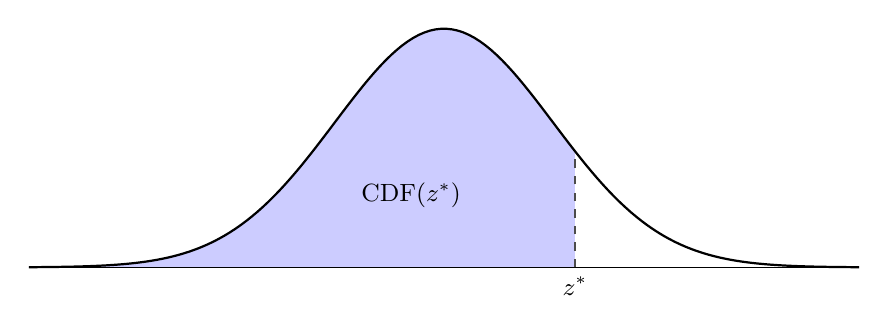
\begin{tikzpicture} % TikZ picture environment
        \begin{axis}[
            % Axis styling for a clean "mini plot"
            axis lines=none, % Hide default axis lines; we'll draw a minimal x-axis manually
            domain=-3.8:3.8, % X-axis range for the plot
            samples=200,     % Number of samples for a smoother curve
            height=5cm,      % Height of the plot area
            width=\linewidth,% Plot takes full width of its minipage container
            ymin=0, ymax=0.45,% Set y-limits to prevent clipping and give some top space
            xtick=\empty, ytick=\empty, % No ticks on axes
            enlarge x limits=false,    % Do not enlarge x-axis limits beyond domain
            clip=false       % Allow nodes (labels) to be placed outside the axis area if needed
        ]
        % Define the value for z* (e.g., 1.2)
        \def\zstar{1.2}

        % Path for the PDF curve (used by fill between, but not drawn itself yet by this command)
        \addplot [draw=none, name path=pdfcurve, domain=-3.8:3.8, samples=100]
            {1/(sqrt(2*pi))*exp(-x^2/2)};
        % Path for the x-axis segment used for filling
        \path [name path=xaxis] (axis cs:-3.8,0) -- (axis cs:3.8,0);

        % Fill the area under the curve from the left up to z_star
        \addplot [fill=blue!20] fill between [
            of=pdfcurve and xaxis, % Specify the paths to fill between
            soft clip={domain=-3.8:\zstar} % Limit the filling range horizontally
        ];
        
        % Plot the PDF curve (thick black line, drawn on top of the fill)
        \addplot [thick, color=black, domain=-3.8:3.8, samples=150] % More samples for smoothness
            {1/(sqrt(2*pi))*exp(-x^2/2)};
        
        % Draw a minimal x-axis line
        \draw [color=black] (axis cs:-3.8,0) -- (axis cs:3.8,0);

        % Draw a vertical dashed line from the x-axis to the curve at z*
        \draw [dashed, color=black!70] (axis cs:\zstar, 0) -- (axis cs:\zstar, {1/(sqrt(2*pi))*exp(-\zstar^2/2)});

        % Label z* on the x-axis
        \node[below, font=\small] at (axis cs:\zstar, 0) {$z^*$};

        % Label "CDF(z*)" in the shaded area
        % Adjust coordinates (axis cs: X, Y) as needed for good placement
        \node[font=\small, align=center] at (axis cs:-0.3, 0.12) {CDF($z^*$)};
        \end{axis}
    \end{tikzpicture}
\end{minipage}% % The '%' is important to avoid unwanted space between minipages
\hfill % Adds flexible horizontal space, pushing minipages apart
\begin{minipage}[t]{0.48\textwidth} % Right column for the "Common Critical Values" table
    \centering
    % Using the original title for the table as requested
    \vspace{1em}
    \textbf{Common Critical Values -- Exact Values} \\ \textbf{(up to the 4th decimal):} \\ 
    \vspace{0.8em} % Adjusted space for potentially longer title
    \small % Make table font smaller to fit comfortably
    \setlength{\tabcolsep}{4pt} % Adjust column separation for the table
    \renewcommand{\arraystretch}{1.3} % Adjust row height for the table
    % Changed from 'array' environment to 'tabular' for better text handling
    \begin{tabular}{|c|c|c|c|c|c|}
        \hline
        CDF & 0.90 & 0.95 & 0.975 & 0.99 & 0.995 \\ \hline
        $z$ & 1.2816 & 1.6449 & 1.9600 & 2.3263 & 2.5758 \\ \hline
    \end{tabular}
\end{minipage}


%=============================================================
% Main CDF table (unchanged)
%=============================================================

\centering{ \textbf{Standard Normal Cumulative Distribution Function (CDF) Table}}

\small

\begin{table}[ht!]
\renewcommand{\arraystretch}{1.2}
\centering
\begin{tabular}{|p{0.05\textwidth}|p{0.05\textwidth}|p{0.02\textwidth}|p{0.05\textwidth}|p{0.05\textwidth}|p{0.02\textwidth}|p{0.05\textwidth}|p{0.05\textwidth}|p{0.02\textwidth}|p{0.05\textwidth}|p{0.05\textwidth}|p{0.02\textwidth}}
\cline{1-2} \cline{4-5} \cline{7-8}  \cline{10-11}
\textbf{z} & \textbf{CDF} &  & \textbf{z} & \textbf{CDF} &  & \textbf{z} & \textbf{CDF} &  & \textbf{z} & \textbf{CDF} &  \\ \cline{1-2} \cline{4-5} \cline{7-8}  \cline{10-11}
-3.05 & 0.0011 &  & -1.50 & 0.0668 &  & 0.05 & 0.5199 &  & 1.60 & 0.9452 &  \\ \cline{1-2} \cline{4-5} \cline{7-8}  \cline{10-11}
-3.00 & 0.0013 &  & -1.45 & 0.0735 &  & 0.10 & 0.5398 &  & 1.65 & 0.9505 &  \\ \cline{1-2} \cline{4-5} \cline{7-8}  \cline{10-11}
-2.95 & 0.0016 &  & -1.40 & 0.0808 &  & 0.15 & 0.5596 &  & 1.70 & 0.9554 &  \\ \cline{1-2} \cline{4-5} \cline{7-8}  \cline{10-11}
-2.90 & 0.0019 &  & -1.35 & 0.0885 &  & 0.20 & 0.5793 &  & 1.75 & 0.9599 &  \\ \cline{1-2} \cline{4-5} \cline{7-8}  \cline{10-11}
-2.85 & 0.0022 &  & -1.30 & 0.0968 &  & 0.25 & 0.5987 &  & 1.80 & 0.9641 &  \\ \cline{1-2} \cline{4-5} \cline{7-8}  \cline{10-11}
-2.80 & 0.0026 &  & -1.25 & 0.1056 &  & 0.30 & 0.6179 &  & 1.85 & 0.9678 &  \\ \cline{1-2} \cline{4-5} \cline{7-8}  \cline{10-11}
-2.75 & 0.0030 &  & -1.20 & 0.1151 &  & 0.35 & 0.6368 &  & 1.90 & 0.9713 &  \\ \cline{1-2} \cline{4-5} \cline{7-8}  \cline{10-11}
-2.70 & 0.0035 &  & -1.15 & 0.1251 &  & 0.40 & 0.6554 &  & 1.95 & 0.9744 &  \\ \cline{1-2} \cline{4-5} \cline{7-8}  \cline{10-11}
-2.65 & 0.0040 &  & -1.10 & 0.1357 &  & 0.45 & 0.6736 &  & 2.00 & 0.9772 &  \\ \cline{1-2} \cline{4-5} \cline{7-8}  \cline{10-11}
-2.60 & 0.0047 &  & -1.05 & 0.1469 &  & 0.50 & 0.6915 &  & 2.05 & 0.9798 &  \\ \cline{1-2} \cline{4-5} \cline{7-8}  \cline{10-11}
-2.55 & 0.0054 &  & -1.00 & 0.1587 &  & 0.55 & 0.7088 &  & 2.10 & 0.9821 &  \\ \cline{1-2} \cline{4-5} \cline{7-8}  \cline{10-11}
-2.50 & 0.0062 &  & -0.95 & 0.1711 &  & 0.60 & 0.7257 &  & 2.15 & 0.9842 &  \\ \cline{1-2} \cline{4-5} \cline{7-8}  \cline{10-11}
-2.45 & 0.0071 &  & -0.90 & 0.1841 &  & 0.65 & 0.7422 &  & 2.20 & 0.9861 &  \\ \cline{1-2} \cline{4-5} \cline{7-8}  \cline{10-11}
-2.40 & 0.0082 &  & -0.85 & 0.1977 &  & 0.70 & 0.7580 &  & 2.25 & 0.9878 &  \\ \cline{1-2} \cline{4-5} \cline{7-8}  \cline{10-11}
-2.35 & 0.0094 &  & -0.80 & 0.2119 &  & 0.75 & 0.7734 &  & 2.30 & 0.9893 &  \\ \cline{1-2} \cline{4-5} \cline{7-8}  \cline{10-11}
-2.30 & 0.0107 &  & -0.75 & 0.2266 &  & 0.80 & 0.7881 &  & 2.35 & 0.9906 &  \\ \cline{1-2} \cline{4-5} \cline{7-8}  \cline{10-11}
-2.25 & 0.0122 &  & -0.70 & 0.2420 &  & 0.85 & 0.8023 &  & 2.40 & 0.9918 &  \\ \cline{1-2} \cline{4-5} \cline{7-8}  \cline{10-11}
-2.20 & 0.0139 &  & -0.65 & 0.2578 &  & 0.90 & 0.8159 &  & 2.45 & 0.9929 &  \\ \cline{1-2} \cline{4-5} \cline{7-8}  \cline{10-11}
-2.15 & 0.0158 &  & -0.60 & 0.2743 &  & 0.95 & 0.8289 &  & 2.50 & 0.9938 &  \\ \cline{1-2} \cline{4-5} \cline{7-8}  \cline{10-11}
-2.10 & 0.0179 &  & -0.55 & 0.2912 &  & 1.00 & 0.8413 &  & 2.55 & 0.9946 &  \\ \cline{1-2} \cline{4-5} \cline{7-8}  \cline{10-11}
-2.05 & 0.0202 &  & -0.50 & 0.3085 &  & 1.05 & 0.8531 &  & 2.60 & 0.9953 &  \\ \cline{1-2} \cline{4-5} \cline{7-8}  \cline{10-11}
-2.00 & 0.0228 &  & -0.45 & 0.3264 &  & 1.10 & 0.8643 &  & 2.65 & 0.9960 &  \\ \cline{1-2} \cline{4-5} \cline{7-8}  \cline{10-11}
-1.95 & 0.0256 &  & -0.40 & 0.3446 &  & 1.15 & 0.8749 &  & 2.70 & 0.9965 &  \\ \cline{1-2} \cline{4-5} \cline{7-8}  \cline{10-11}
-1.90 & 0.0287 &  & -0.35 & 0.3632 &  & 1.20 & 0.8849 &  & 2.75 & 0.9970 &  \\ \cline{1-2} \cline{4-5} \cline{7-8}  \cline{10-11}
-1.85 & 0.0322 &  & -0.30 & 0.3821 &  & 1.25 & 0.8944 &  & 2.80 & 0.9974 &  \\ \cline{1-2} \cline{4-5} \cline{7-8}  \cline{10-11}
-1.80 & 0.0359 &  & -0.25 & 0.4013 &  & 1.30 & 0.9032 &  & 2.85 & 0.9978 &  \\ \cline{1-2} \cline{4-5} \cline{7-8}  \cline{10-11}
-1.75 & 0.0401 &  & -0.20 & 0.4207 &  & 1.35 & 0.9115 &  & 2.90 & 0.9981 &  \\ \cline{1-2} \cline{4-5} \cline{7-8}  \cline{10-11}
-1.70 & 0.0446 &  & -0.15 & 0.4404 &  & 1.40 & 0.9192 &  & 2.95 & 0.9984 &  \\ \cline{1-2} \cline{4-5} \cline{7-8}  \cline{10-11}
-1.65 & 0.0495 &  & -0.10 & 0.4602 &  & 1.45 & 0.9265 &  & 3.00 & 0.9987 &  \\ \cline{1-2} \cline{4-5} \cline{7-8}  \cline{10-11}
-1.60 & 0.0548 &  & -0.05 & 0.4801 &  & 1.50 & 0.9332 &  & 3.05 & 0.9989 &  \\ \cline{1-2} \cline{4-5} \cline{7-8}  \cline{10-11}
-1.55 & 0.0606 &  & -0.00 & 0.5000 &  & 1.55 & 0.9394 &  &  &  &  \\ \cline{1-2} \cline{4-5} \cline{7-8}  \cline{10-11}
\end{tabular}
\end{table}


\textbf{Reminders:}
\begin{itemize}
    \item Note that $P(Z\geq z^*) = 1 -  CDF(z^*)$.
    \item Because the $z$--distribution is symmetrical: $CDF(-|z^*|) = 1 - CDF(|z^*|)$. 
    \begin{itemize}
        \item For instance, $CDF(-1.96) = 1 - CDF(1.96)=0.025$.
        \item For instance, $CDF(-1.6449) = 1 - CDF(1.6449)=0.05$.
    \end{itemize}
    \item Remember: $P(a < Z < b) = CDF(b) - CDF(a)$.
\end{itemize}


\end{document}


\documentclass[letterpaper]{article} % Corrected from letterpage
\usepackage[top=0.15in, left=0.1in, right=0.1in, bottom=1in]{geometry}
\usepackage{amsmath,amssymb,array,multirow}
\usepackage{tikz}
\usepackage{pgfplots}
\pgfplotsset{compat=1.18} % Use a recent compatibility version for pgfplots
\setlength{\arrayrulewidth}{0.1pt}

\begin{document}
\pagenumbering{gobble}



\vspace{3em} % Space between the top two-column section and the main CDF table title

% --- Original Main Title and Large CDF Table ---
\centering % Center the main title
\textbf{Standard Normal Cumulative Distribution Function (CDF) Table}
\vspace{1em} % Space after the main title, before the large table

\small % This was already here, applies to the large CDF table

\begin{table}[ht!] % The original table float environment
\renewcommand{\arraystretch}{1.2} % This was already here for this table
\centering % This was already here for this table
\begin{tabular}{|p{0.10\textwidth}|p{0.13\textwidth}|p{0.02\textwidth}|p{0.10\textwidth}|p{0.13\textwidth}|p{0.02\textwidth}|p{0.10\textwidth}|p{0.13\textwidth}|}
\cline{1-2} \cline{4-5} \cline{7-8}
\textbf{z} & \textbf{CDF} &  & \textbf{z} & \textbf{CDF} &  & \textbf{z} & \textbf{CDF} \\ \cline{1-2} \cline{4-5} \cline{7-8}
-3.05 & 0.0011 &  & -1.00 & 0.1587 &  & 1.05 & 0.8531 \\ \cline{1-2} \cline{4-5} \cline{7-8}
-3.00 & 0.0013 &  & -0.95 & 0.1711 &  & 1.10 & 0.8643 \\ \cline{1-2} \cline{4-5} \cline{7-8}
-2.95 & 0.0016 &  & -0.90 & 0.1841 &  & 1.15 & 0.8749 \\ \cline{1-2} \cline{4-5} \cline{7-8}
-2.90 & 0.0019 &  & -0.85 & 0.1977 &  & 1.20 & 0.8849 \\ \cline{1-2} \cline{4-5} \cline{7-8}
-2.85 & 0.0022 &  & -0.80 & 0.2119 &  & 1.25 & 0.8944 \\ \cline{1-2} \cline{4-5} \cline{7-8}
-2.80 & 0.0026 &  & -0.75 & 0.2266 &  & 1.30 & 0.9032 \\ \cline{1-2} \cline{4-5} \cline{7-8}
-2.75 & 0.0030 &  & -0.70 & 0.2420 &  & 1.35 & 0.9115 \\ \cline{1-2} \cline{4-5} \cline{7-8}
-2.70 & 0.0035 &  & -0.65 & 0.2578 &  & 1.40 & 0.9192 \\ \cline{1-2} \cline{4-5} \cline{7-8}
-2.65 & 0.0040 &  & -0.60 & 0.2743 &  & 1.45 & 0.9265 \\ \cline{1-2} \cline{4-5} \cline{7-8}
-2.60 & 0.0047 &  & -0.55 & 0.2912 &  & 1.50 & 0.9332 \\ \cline{1-2} \cline{4-5} \cline{7-8}
-2.55 & 0.0054 &  & -0.50 & 0.3085 &  & 1.55 & 0.9394 \\ \cline{1-2} \cline{4-5} \cline{7-8}
-2.50 & 0.0062 &  & -0.45 & 0.3264 &  & 1.60 & 0.9452 \\ \cline{1-2} \cline{4-5} \cline{7-8}
-2.45 & 0.0071 &  & -0.40 & 0.3446 &  & 1.65 & 0.9505 \\ \cline{1-2} \cline{4-5} \cline{7-8}
-2.40 & 0.0082 &  & -0.35 & 0.3632 &  & 1.70 & 0.9554 \\ \cline{1-2} \cline{4-5} \cline{7-8}
-2.35 & 0.0094 &  & -0.30 & 0.3821 &  & 1.75 & 0.9599 \\ \cline{1-2} \cline{4-5} \cline{7-8}
-2.30 & 0.0107 &  & -0.25 & 0.4013 &  & 1.80 & 0.9641 \\ \cline{1-2} \cline{4-5} \cline{7-8}
-2.25 & 0.0122 &  & -0.20 & 0.4207 &  & 1.85 & 0.9678 \\ \cline{1-2} \cline{4-5} \cline{7-8}
-2.20 & 0.0139 &  & -0.15 & 0.4404 &  & 1.90 & 0.9713 \\ \cline{1-2} \cline{4-5} \cline{7-8}
-2.15 & 0.0158 &  & -0.10 & 0.4602 &  & 1.95 & 0.9744 \\ \cline{1-2} \cline{4-5} \cline{7-8}
-2.10 & 0.0179 &  & -0.05 & 0.4801 &  & 2.00 & 0.9772 \\ \cline{1-2} \cline{4-5} \cline{7-8}
-2.05 & 0.0202 &  & 0.00 & 0.5000 &  & 2.05 & 0.9798 \\ \cline{1-2} \cline{4-5} \cline{7-8}
-2.00 & 0.0228 &  & 0.05 & 0.5199 &  & 2.10 & 0.9821 \\ \cline{1-2} \cline{4-5} \cline{7-8}
-1.95 & 0.0256 &  & 0.10 & 0.5398 &  & 2.15 & 0.9842 \\ \cline{1-2} \cline{4-5} \cline{7-8}
-1.90 & 0.0287 &  & 0.15 & 0.5596 &  & 2.20 & 0.9861 \\ \cline{1-2} \cline{4-5} \cline{7-8}
-1.85 & 0.0322 &  & 0.20 & 0.5793 &  & 2.25 & 0.9878 \\ \cline{1-2} \cline{4-5} \cline{7-8}
-1.80 & 0.0359 &  & 0.25 & 0.5987 &  & 2.30 & 0.9893 \\ \cline{1-2} \cline{4-5} \cline{7-8}
-1.75 & 0.0401 &  & 0.30 & 0.6179 &  & 2.35 & 0.9906 \\ \cline{1-2} \cline{4-5} \cline{7-8}
-1.70 & 0.0446 &  & 0.35 & 0.6368 &  & 2.40 & 0.9918 \\ \cline{1-2} \cline{4-5} \cline{7-8}
-1.65 & 0.0495 &  & 0.40 & 0.6554 &  & 2.45 & 0.9929 \\ \cline{1-2} \cline{4-5} \cline{7-8}
-1.60 & 0.0548 &  & 0.45 & 0.6736 &  & 2.50 & 0.9938 \\ \cline{1-2} \cline{4-5} \cline{7-8}
-1.55 & 0.0606 &  & 0.50 & 0.6915 &  & 2.55 & 0.9946 \\ \cline{1-2} \cline{4-5} \cline{7-8}
-1.50 & 0.0668 &  & 0.55 & 0.7088 &  & 2.60 & 0.9953 \\ \cline{1-2} \cline{4-5} \cline{7-8}
-1.45 & 0.0735 &  & 0.60 & 0.7257 &  & 2.65 & 0.9960 \\ \cline{1-2} \cline{4-5} \cline{7-8}
-1.40 & 0.0808 &  & 0.65 & 0.7422 &  & 2.70 & 0.9965 \\ \cline{1-2} \cline{4-5} \cline{7-8}
-1.35 & 0.0885 &  & 0.70 & 0.7580 &  & 2.75 & 0.9970 \\ \cline{1-2} \cline{4-5} \cline{7-8}
-1.30 & 0.0968 &  & 0.75 & 0.7734 &  & 2.80 & 0.9974 \\ \cline{1-2} \cline{4-5} \cline{7-8}
-1.25 & 0.1056 &  & 0.80 & 0.7881 &  & 2.85 & 0.9978 \\ \cline{1-2} \cline{4-5} \cline{7-8}
-1.20 & 0.1151 &  & 0.85 & 0.8023 &  & 2.90 & 0.9981 \\ \cline{1-2} \cline{4-5} \cline{7-8}
-1.15 & 0.1251 &  & 0.90 & 0.8159 &  & 2.95 & 0.9984 \\ \cline{1-2} \cline{4-5} \cline{7-8}
-1.10 & 0.1357 &  & 0.95 & 0.8289 &  & 3.00 & 0.9987 \\ \cline{1-2} \cline{4-5} \cline{7-8}
-1.05 & 0.1469 &  & 1.00 & 0.8413 &  & 3.05 & 0.9989 \\ \cline{1-2} \cline{4-5} \cline{7-8}
\end{tabular}
\end{table}

% The original \vspace{2em} and "Common Critical Values" table that were here are now moved to the top.

\end{document}
